\section{Chisel}
\label{sec:chisel}
Chisel is a domain specific language embedded in the Scala
programming language so it is really just a library of Scala functions
and data structures. Someone writing Chisel code is essentially writing a Scala
program that uses the provided functions and data structures to
construct hardware. This rest of this section introduces the core
components of the Chisel hardware construction language; readers
interested in a more a detailed specification of Chisel should consult
the Chisel manual. 

\subsection{Node}

\begin{figure}
\centering
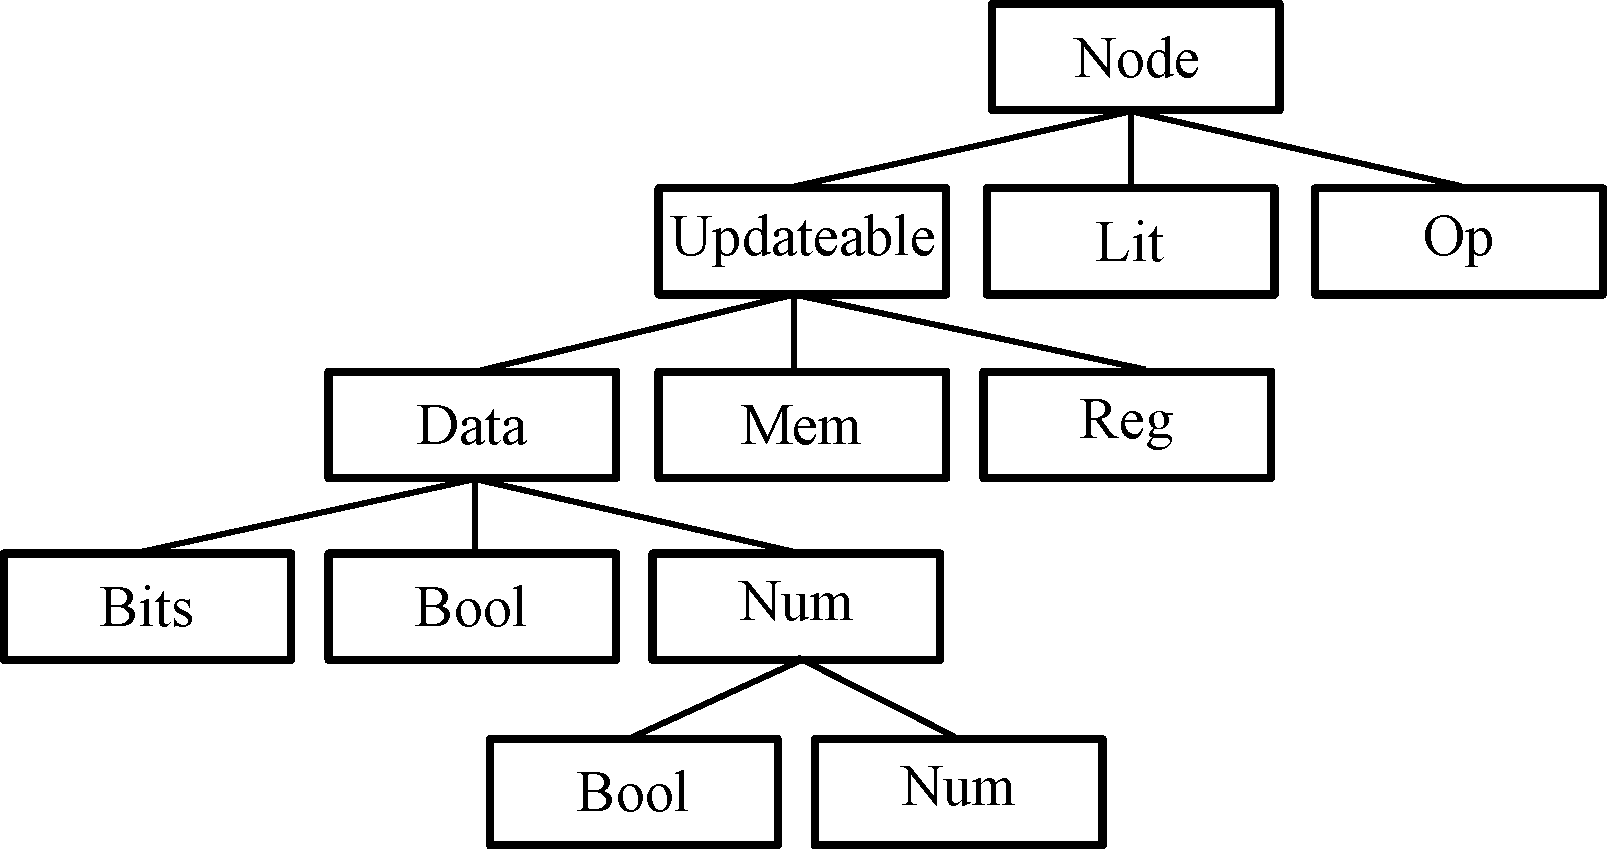
\includegraphics[width=0.75\textwidth]{figures/hierarchy.pdf}
\caption{Chisel Node Hierarchy}
\label{fig:hier}
\end{figure}

\begin{figure}
\centering
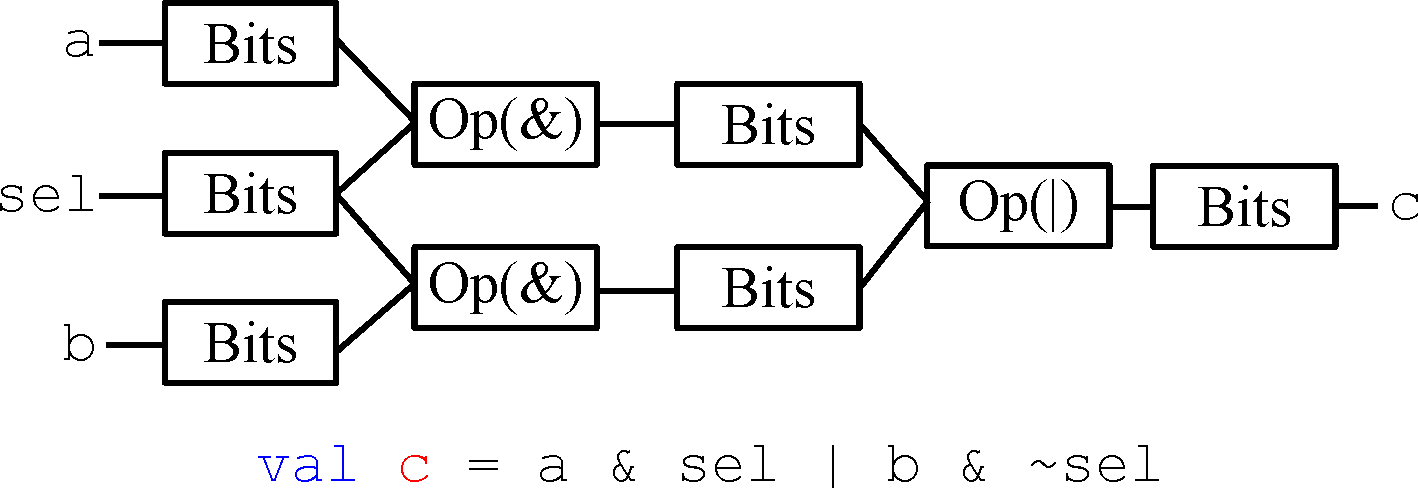
\includegraphics[width=0.75\textwidth]{figures/mux.pdf}
\caption{2-Input Mux}
\label{fig:mux}
\end{figure}

Hardware circuits are represented in Chisel as directed graphs of
{\tt Nodes}, which are the base class from which all circuit elements are
derived. Figure~\ref{fig:hier} shows the Chisel class
hierarchy. Figure~\ref{fig:mux} shows an example snippet of Chisel
code and the corresponding directed graph of {\tt Nodes} that is constructed.

{\bf Types}. Chisel has its own type system that is maintained
independent of the Scala type system. Figure~\ref{fig:hier} shows the
Chisel data types and their hierarchy (everything rooted at the 
{\tt Data Node}. Bits is used to represent raw collection of bits, Bool is used
for logical operations, and Num is used for arithmetic. Note that Num
has two subclasses, Fix and UFix which are used for signed and
unsigned operations respectively.

{\bf Literals} The {\tt Lit Node} works in conjunction with type {\tt Nodes} to
represent literals. True and false literals are represented as Bools
connected to {\tt Lit Nodes} 1 and 0 respectively. Arbitrary bit strings are
represented with {\tt Bits Nodes} and numbers are represented with
{\tt Fix} and {\tt UFix Nodes}, connected to {\tt Lit Nodes} with the
appropritate value.

{\bf Arithmetic and Logic}. Arithmetic and logic operations
are represented with {\tt Op Nodes}. Chisel supports the operations defined
in Figure~\ref{fig:typedef}. Note that the arithmetic and logic
functions are Chisel functions defined between type {\tt Nodes}. Invoking
those functions will invoke the constructor for an {\tt Op Node} with the
appropriate input parameters.

{\bf Registers} The {\tt Reg Node}, Chisel most basic state element,
represents a positive-edge-triggered flip-flop. {\tt Reg Nodes}, unlike the
previous {\tt Nodes}, are manually instantiated by the
user. Figure~\ref{fig:reg} shows the different ways that a {\tt Reg} can be
instantiated.

{\bf Memories} {\tt Mem Nodes} are used to represent random access
memories. These memories can be accesssed with either {\tt Bits} or
{\tt UFix Nodes}. Writes to these memories are positive-edge-triggered while
reads can be either combination or positive-edge-trigerred.

\subsection{Component}
In addition to {\tt Nodes}, Chisel also provides {\tt Components} which users can
use to organize their directed graph of {\tt Nodes} into subgraphs, adding a
hierarchical structure to their hardware. Figure~\ref{fig:comp} shows
the {\tt Component} API. Figure~\ref{fig:mux} shows example Chisel
implementation of a 4 input mux.

{\bf Interfaces} When defining a new Component, users have to fill out
the {\tt io} field which is the input-output interface that
Components expose to each other. An input or output node in Chisel is
represented with a Type Node where the direction field is set to
either {\tt INPUT} or {\tt OUTPUT}. Input and output nodes can be
collected into Bundles, which are functionally similar to to C
structs, for better organization. 

{\bf Wiring} Chisel provides two different ways for connecting
Components together. {\tt :=} is used for connections goings from
right to left while {\tt <>} is used for connections that go in both directions.

\subsection{Backend}
\cite{Bachrach:2012}
